\chapter{Introduction}
\label{ch:introduction}
The use of scientific computing to study the Qur'an is still in its early stages within the field of Islamic Studies. This is evident from the fact that no book has yet been written on this subject. This thesis hopes to fill at least some of these gaps. That said, the readers of this paper may come from Islamic Studies and Statistical Science, as well as from other fields of science dealing with statistical modeling and machine learning. Therefore, it is necessary to provide background on topics from both fields to help readers appreciate the synergy between these disciplines.

\section{Background}
The Qur'\=an or \arb[trans]{al-qur'An} \arb{al-qur'An} meaning \textit{the recitation}, the holy book of Islam, is revered by 1.9 billion (according to 2020 projection of \shortciteA[p.~13]{pewresearch}) Muslims across the globe as the literal words of God. Muslims believed that the Qur'\=an was gradually revealed (Qur'\=an 25:32) to Prophet Muhammad \arb{\arbmark{slm}} through angel \arb[trans]{jibrIl} \arb{jibrIl} or Gabriel (Qur'\=an 2:97). The Qur'\=an contains 77,429 Arabic words in total, which covers only 56 percent of the Greek New Testament which has 138,020 words in total \cite[p.~11]{sinai2017}. 

The Qur'\=an is divided into \arb[trans]{sUwar} \arb{sUwar} (\textit{plural} of \arb[trans]{sUraT} \arb{sUraT}) which are the equivalent of chapters, each containing \arb[trans]{'AyAt} \arb{'AyAt} (\textit{plural} of \arb[trans]{'AyaT} \arb{'AyaT} meaning \textit{signs}), which are the equivalent of verses. The \arb[trans]{sUwar} \arb{sUwar} are not arranged in chronological order like the Bible's books and chapters, but rather arranged in monotonically decreasing length of number of verses after the first \arb[trans]{sUraT} \arb{sUraT} (\textit{see} Figure \ref{fig:ayah_word_count}). The \arb[trans]{sUwar} \arb{sUwar} of the Qur'\=an can be categorized into two types: the \arb[trans]{makkiyyaT} \arb{makkiyyaT} (Meccan) and \arb[trans]{madaniyyaT} \arb{madaniyyaT} (Medinan). The categories refer to the geographical location of where the \arb[trans]{sUraT} \arb{sUraT} was revealed to Prophet Muhammad \arb{\arbmark{slm}}. Figure \ref{fig:ayah_word_count} shows the groupings of the \arb[trans]{sUwar} \arb{sUwar}. Note that some of the \arb[trans]{sUwar} \arb{sUwar} have mixed geographical locations\footnote{\textit{see} list of the location in \url{https://tanzil.net/docs/revelation_order}}, that is, a few of the \arb[trans]{'AyAt} \arb{'AyAt} in it were revealed in other geographical location apart from the geographical location of the rest of the \arb[trans]{'AyAt} \arb{'AyAt}. Therefore, the categorization in Figure \ref{fig:ayah_word_count} highlights the geographical location of the majority of the \arb[trans]{'AyAt} \arb{'AyAt} in the \arb[trans]{sUraT} \arb{sUraT}.

\begin{figure}[!b]
    \centering
    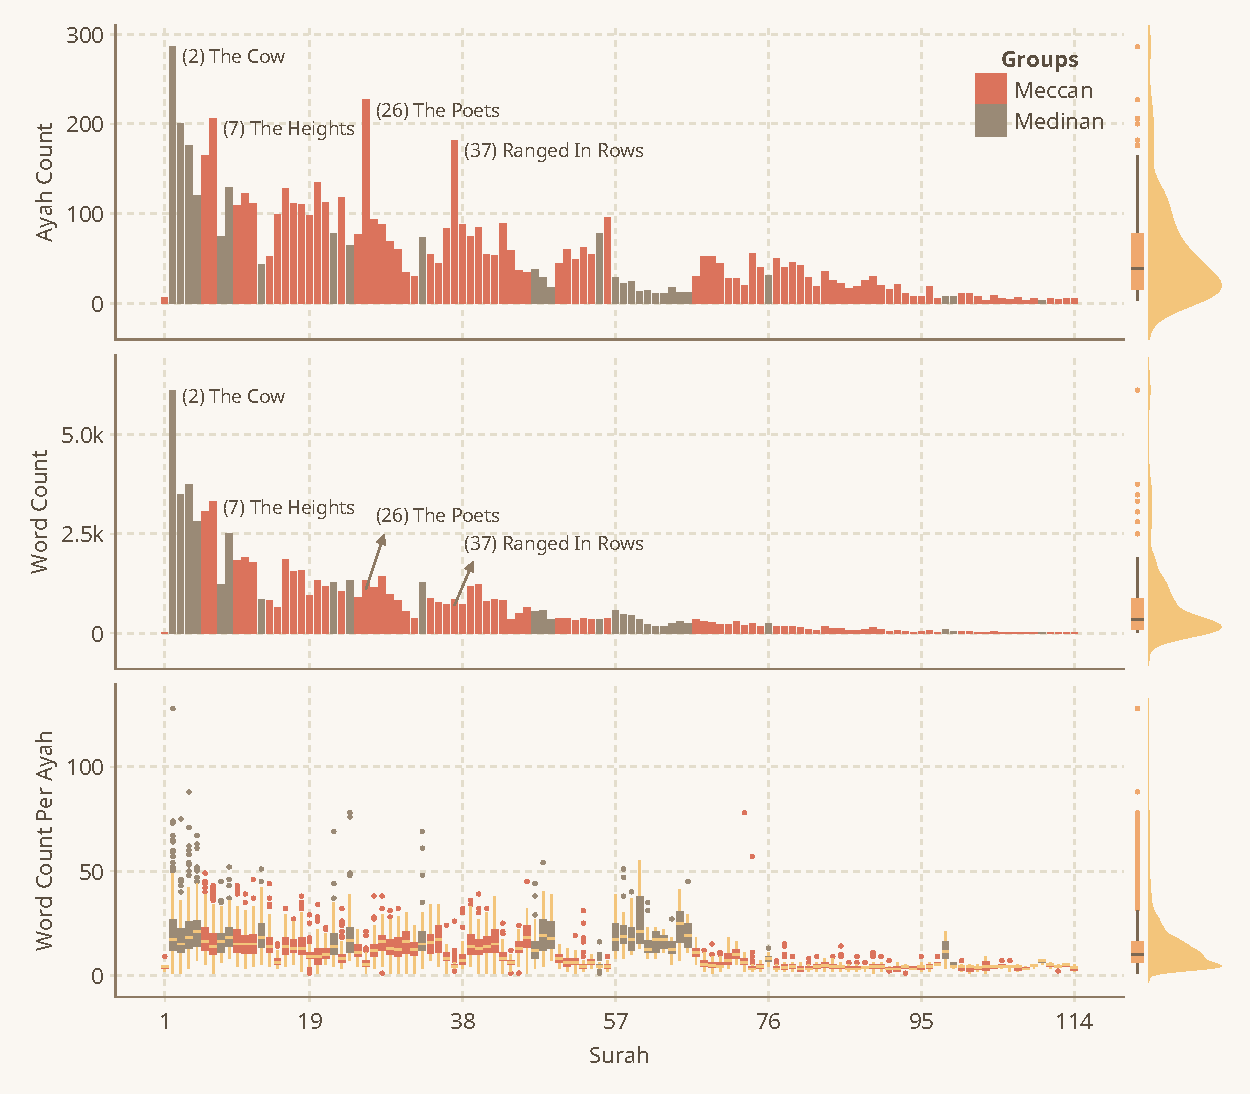
\includegraphics[width=\textwidth]{img/plot1.pdf}
    \caption{Statistics of the words and \arb[trans]{'AyAt} \arb{'AyAt} (verses) of the Qur'\=an}
    \label{fig:ayah_word_count}
\end{figure}

Attempts at understanding the Qur'\=an by Qur'\=anic scholars were mostly done through the manual process, that is, studying the scriptures by going through its content manually line-by-line or one-at-a-time. However, with the advent of computers, some researchers have started using it to aid in their study. The first known to have used computers for studying the Qur'\=an was likely Rashad Khalifa in 1968\footnote{\url{https://www.masjidtucson.org/quran/miracle/a_profound_miracle_sura68nun133.html}}, where he studied the significance of the mysterious initials at the beginning of some \arb[trans]{sUwar} \arb{sUwar}. Rashad uploaded the Qur'\=an into his computer by transliterating the Arabic letters and other Qur'\=anic orthographies into Roman letters and symbols that the computer can easily parse. This approach of using computers to find new insights is more common in the field of science, and it was new to the field of Qur'\=anic studies.

Indeed, to proceed with the use of scientific computing, the Qur'\=an will be treated as the main data that needs to be analyzed using a scientific process called Natural Language Processing (NLP), a branch of Machine Learning (ML) that aims to understand natural languages, including Arabic. To instruct the computer to do statistical analyses and ML, one needs to use a \textit{software application} or a formal\footnote{"formal" because these languages were invented by man for particular purpose, in this case to communicate with computers} language called \textit{programming language}. There are several programming languages that the computer can understand. The popular one for researchers in the field of sciences are Python \cite{van1995python}, R \cite{rprogramming}, and sometimes Julia \shortcite{Julia2017}. These programming languages are used to construct instructions for computers. Therefore, if the data is the Qur'\=an, then there should be a way to interface with it using any of these programming languages; or alternatively, there should be a way to upload it into the chosen programming language and encode the Arabic letters into something that can be easily parsed by the computers, like what Rashad \mbox{Khalifa} did. Having said that, there are indeed some programming languages with libraries or packages for interfacing with the Qur'\=an, and this is true for Python, R, and \mbox{Julia}. For this study, only Julia programming language is used. The ruling is that Julia will be used for interfacing with the Qur'\=an's texts since the library for doing this has more features \cite<\textit{see}>{asaad2021qurantree} compared to that available in R and in Python. The said Julia library is the QuranTree.jl\footnote{\url{https://alstat.github.io/QuranTree.jl/stable/}}. QuranTree.jl is based on Tanzil\footnote{\url{https://tanzil.net/download/}} for the Qur'\=anic Arabic texts, and \citeA{dukes-habash-2010-morphological} for morphological annotation, which both libraries from R and Python do not have in terms of morphological annotations from \citeA{dukes-habash-2010-morphological}. 

Given the programming languages, next is to understand how Statistics and Machine Learning can help in studying the Qur'\=an. Statistics is a branch of science that aims to study features or characteristics of data generated from random phenomena. The findings of statistical analyses can then be used to make decisions, draw conclusions, or make predictions about the general population of the data or general characteristics of the data. Machine Learning, or ML, on the other hand, is a branch of Artificial Intelligence (AI) that heavily intersects with Statistics, albeit with distinct differences as well. Both Statistics and ML aim to characterize data by learning its features, but ML researchers have been focusing on complex models that are often inspired by simpler models from Statistics. Therefore, one can think of Statistics as one of the fundamentals of ML.

One of the goals of Statistics and Machine Learning is to summarize all of the learned features of the data into a hypothesized equation or mathematical formula by optimizing the parameters or weights of this equation or formula to capture \textit{most}\footnote{Not all characteristics of the data can be captured by the model, and those that are not captured are called the errors. The goal is to minimize these errors to a tolerable level.} of the characteristics of the data. The idea stems from the fact that any data point is simply a sum of its components, which are factors known to affect the data point. For example, the volume of orders in a restaurant is dependent on the time of day. More orders are expected during lunch and dinner. Hence, volume of orders as data points can be derived from the sum of factors such as time of day, and also day of the week (assuming more orders during weekends or weekdays). Therefore, from this example, any data point is affected by factors that can be translated into mathematical formulation such that their sum results in the data points we want, like the volume of orders. This is why hypothesized mathematical equations or formulas are used for summarizing the features and capturing the characteristics of data. It is called a \textit{hypothesized equation} since the researcher is the one who decides which family of equations best describes the characteristics of the data. Many possible mathematical formulae can be constructed, but not all can be used to describe the data, which is why the researcher must decide. Those equations that can be used for understanding the data are special enough that they are referred to as \textit{models}. Mathematically and in general, a model can be related to the data as follows:
\begin{equation}\label{eq:general_model}
    y=h(x|\boldsymbol{\theta})+\varepsilon,
\end{equation}
where $h(x|\boldsymbol{\theta})$ is the hypothesized model taking the input data $x$ (from the examples discussed above, these are the values of the factors affecting the volume of orders), where $x\in\mathscr{X}$ (read as $x$ is an element of $\mathscr{X}$; from the examples discussed above, $\mathscr{X}$ is the set containing all values of the factors mentioned), and outputs a target data $y$ (from the examples discussed above, this is the volume of orders), where $y\in\mathscr{Y}$. Therefore, $h:\mathscr{X}\rightarrow\mathscr{Y}$ (read as $h$ is mapping from $\mathscr{X}$ to $\mathscr{Y}$), that is, $h$ maps the factors or features into the set of the target variable $y$. The $\varepsilon$ is the error that the hypothesized model $h(x|\boldsymbol{\theta})$ cannot capture even after finding the best configuration of its parameter $\boldsymbol{\theta}$. Ideally, the error or \textit{residual} or sometimes called \textit{innovation}, $\varepsilon$, should exhibit \textit{random noise} for us to say that the hypothetical model $h(x|\boldsymbol{\theta})$ has captured the core characteristics of the data $(x,y)$ well. These random noises are data points that could have come from other factors that are not available in the given data, $(x,y)$. Therefore, the idea of modeling is to find the optimal value of $\boldsymbol{\theta}$ such that the error between the actual data (represented by $y$ below) and the predicted one $\hat{y}$, is as small as possible or tolerable:
\begin{equation}
    \varepsilon:=y-\hat{y}=y-h(x|\boldsymbol{\theta}).
\end{equation}

To help understand the concept of modeling, and relate it to the fashion industry, which the author assumes most readers are familiar with, a model in a fashion industry is responsible for representing the characteristics of the target customers (in Equation \ref{eq:general_model} this is $y$). Therefore, for a clothing company, they hire Asian models (in Equation \ref{eq:general_model}, this is $\hat{y}:=h(x|\boldsymbol{\theta})$) to target Asian customers (in Equation \ref{eq:general_model} this is $y$). So that, when these models wore the clothes sold by the said company, the potential customer will more or less be able to relate to the model, and be able to imagine themselves wearing that same clothes as well, which help them incline to buying the said clothing. The model, therefore, does not necessarily have the looks of every target Asian customers, but at least in terms of height, skin tone, hair, and other common Asian features, the model will likely have it, or at least the difference is more or less minimal (in Equation \ref{eq:general_model}, the difference is represented by $\varepsilon:=y-\hat{y}$). The question now is, what are the benefits that this model can bring to the clothing company? Well, the clothing company will be able to create products that are tailored to their Asian customers using the said model, since the company will have the right baseline measurements needed. Relating this analogy to the technical concept discussed earlier, you can think of the target customers as the
real or actual data (in Equation \ref{eq:general_model} this is $y$), and the model as the same technical term use in Machine Learning and Statistics (in Equation \ref{eq:general_model} this is $\hat{y}:=h(x|\boldsymbol{\theta})$), but this time this technical model is expected to capture the characteristics of the real data analogous to fashion model that is expected to capture the characteristics of the target customer. This Statistical or Machine Learning model brings the following benefits: researchers will be able to study the real data by simply using the model to answer questions that are not available in the sampled real data.

\section{Rationale of the Study}\label{sec:rationale}
Having understood the background of this study, let's turn our attention to the rationale. When it comes to modeling the characteristics of any data, there are several ways to do it, and it all depends on the questions one would like to answer. Apart from this, it also depends on the richness of the data. This is true for the Qur'\=an as well. The rich morphological annotations done by \citeA{dukes-habash-2010-morphological} has opened a lot of opportunities for statistical analyses. It is even hard to decide on where to start since this morphological data has not been extensively studied yet, at least based from the survey of \shortciteA{DarwishHabash2021} and \shortciteA{bashir2023arabic}, and apart from the work of  \shortciteA{dukes2013supervised} and \shortciteA{dukes2010online} on the dependency graph of the morphological annotations of their original work \cite{dukes-habash-2010-morphological}. Most of the NLP studies done on the Qur'\=an have revolved around corpus creation on annotations of mophological features of the Qur'\=an \shortcite{dukes-habash-2010-morphological}, Qur'\=an's pronouns annotations \shortcite{sharaf2012}, the \arb[trans]{'AyAt} \arb{'AyAt} similarity annotations \shortcite{sharaf2012b}, and comparative analyses of corpora \shortcite{sabtan2017morphological}; Qur'\=an's stemming system \shortcite{thabet2004} and its tokenization\footnote{\textit{See} Section \ref{sec:text_tokenization}} \shortcite{thabet2005}; thematic clustering\footnote{\textit{See} Section \ref{sec:method_thematic_analysis}} of some \arb[trans]{sUwar} \arb{sUwar} \shortcite{siddiqui2013, alhawarat2015extracting}; semantic techologies for improved keyword search in the Qur'\=an \shortcite{afzal2019semantically}, and criterias for evaluating the search algorithms \shortcite{alqahtani2017evaluation}; Qur'\=an's recitation validation through speech recognition \shortcite{ahsiahNoor2013, abroNaqvi2012,ahmed2017verification}; Qur'\=an's authorship analyses in comparison to Prophet Muhammad's \arb{\arbmark{slm}} sayings or statements; Qur'\=an's grammatical analyses by predicting the parts-of-speech (POS) \shortcite{ELAFFENDI202135}, \arb[trans]{'i`rAb} \arb{'i`rAb}\footnote{Refers to the inflectional system used to indicate the grammatical case, mood, and other syntactical features of words, particularly nouns, pronouns, adjectives, and verbs.} modeling through enhanced context-free grammar \shortcite{MANNAA20228909}; Word embedding\footnote{\textit{See} Section \ref{sec:word-embeddings}} models for the Qur'\=an, such as the use of doc2vec based vectorization of the \arb[trans]{'AyAt} \arb{'AyAt} \shortcite{ALSHAMMERI2021351}, and other word embedding methods trained on different Islamic texts like \arb[trans]{'a.hAdI_t} \arb{'a.hAdI_t}\footnote{Plural of \arb[trans]{hadI_t} \arb{hadI_t}, which means the recorded words and practices of Prophet Muhammad \arb{\arbmark{slm}}} \shortcite{aliMaged2020}, and the use of Bidirectional Encoding Representation from Transformers\footnote{\textit{See} Section \ref{sec:bert}} (BERT) like CL-AraBERT \shortcite{MALHAS2022103068}; and Qur'\=an's text classification of \arb[trans]{'AyAt} \arb{'AyAt} into their corresponding \arb[trans]{sUraT} \arb{sUraT} \shortcite{al2005statistical}, and into their place of revelation \shortcite{nassourou2011}.

Among the studies mentioned above on the application of NLP to the Qur'\=an, including those surveyed by \shortciteA{DarwishHabash2021} and \shortciteA{bashir2023arabic}, none has looked into the \textit{rhythmic analysis}. In particular, how statistical analyses can be used to study the \textit{rhythmic patterns} of the Qur'\=an. This is the most prevalent feature of the Qur'\=an, in that it rhymes from the very first chapter all the way to the last. This unique characteristics can be easily confirmed by simply searching on YouTube\footnote{\url{https://www.youtube.com/}} for Qur'anic recitation of say \arb[trans]{sUraTu 'l-baqaraT} \arb{sUraTu 'l-baqaraT}, the second chapter of the Qur'an. This unique characteristics separates this book from the rest (more on this on Chapter \ref{ch:quran_history} of this paper), but this obvious feature of the Qur'an has never been analyzed statistically. This is the first paper to the best knowledge of the author to do so. 

Moving on, some papers did not use NLP to analyze the Qur'\=an's texts, instead they studied the statistical profile of the \arb[trans]{'asbAb 'alnuzUl} \arb{'asbAb 'alnuzUl} (the occasions or circumstances of revelation) of each \arb[trans]{sUraT} \arb{sUraT}, which can either be a \arb[trans]{makkiyyaT} \arb{makkiyyaT} (Meccan) or \arb[trans]{madaniyyaT} \arb{madaniyyaT} (Medinan). For example, the work of \shortciteA{Surras2008StatisticalPO} studied the statistics of the said types of \arb[trans]{suwar} \arb{suwar}, by looking at the count of word-size, \arb[trans]{'AyAt} \arb{'AyAt}-size by characters, and \arb[trans]{'AyAt} \arb{'AyAt}-size by words, and then using frequency distribution and other statistics (mean, standard deviation, coefficient of variation) to understand its profile. This work was further extended by \cite{Hasan2022NumericalSO} using data from Adam's Qur'\=an Code Software\footnote{\url{http://www.heliwave.com/?i=1}, retrieved May 2025}. The findings of the said paper is that the average number of \arb[trans]{'AyAt} \arb{'AyAt}, words, and letters or characters in \arb[trans]{madaniyyaT} \arb{madaniyyaT} are higher than in \arb[trans]{makkiyyaT} \arb{makkiyyaT}. However, both papers were only limited to basic statistical analysis, and has not looked into relations of some of these statistics that will provide insights into the structural design of the Qur'\=an.

Furthermore, the rich morphological annotations done by \citeA{dukes-habash-2010-morphological} has opened up many opportunities as emphasized above. However, none has looked into studing these morphological data of the Qur'\=an. The work of \citeA{asaad2021qurantree} has further made it accessible to many researchers by providing the users with a library in Julia programming language, which is a high-level language that is easier to understand than Java programming language---the software developed by \citeA{dukes-habash-2010-morphological} for the said data. Among the papers on morphological analysis, \citeA{Hadi_2023} analyzed the morphology of selected \arb[trans]{'AyAt} \arb{'AyAt}, starting from \arb[trans]{sUraTu 'l-kaw_tari} \arb{sUraTu 'l-kaw_tari} to \arb[trans]{sUraTu 'l-nAsi} \arb{sUraTu 'l-nAsi}, but the said study focused only on describing the morphological features of the words in the said \arb[trans]{suwar} \arb{suwar} and nothing else. To the best knowledge of the author, none has yet looked into the said data and did analysis on it.

In addition, the Corpus Coranicum\footnote{\url{https://corpuscoranicum.de/en}} project from Germany, overseen by Angelika Neuwirth, has brought new datasets for extant manuscripts supplementing the digitized Qur'\=an data. This exciting project has extensive extant manuscripts of the Qur'\=an, where a good amount of which have been radiocarbon dated. The methodology of this radiocarbon dating is discussed by \cite{Radiocarbon14CDatingofQurnManuscripts}. Some recent papers on Qur'\=anic studies such as the work of \cite{sidky2020} have used the said resources for studying the regionality of Qur'\=anic Codices, where upon inspection of some manuscripts from the Corpus Coranicum indicated that the findings are more or less consistent with claims of Muslim's sources on the codices sent out by Uthman ibn Affan \arb{`u_tmAnu bnu `affAn} in the year 645 CE to different regions. This paper will make use of the extant manuscripts from the said projects as well to supplement the computational findings. In comparison to Biblical study, there is no online resources yet available for Bible's extant manuscripts to the best knowledge of the author.

Finally, there is no study yet that used statistical and computational methodology for the \textit{concentrism theory} proposed by \shortcite{farrin2014structure}. The said author suggested that the Qur'\=an follows a symmetric structural characteristics, with \textit{concentric} symmetry as the prevalent pattern in the Qur'\=an. Indeed, no paper yet has come up with a mathematical formulation for finding concentric patterns objectively.

Lastly, the recent advances in Artificial Intelligence have led to language models for Arabic as well. These language models can be used for analyzing natural languages quite accurately. Among these is the CL-AraBERT language model, which is an AraBERT language model but fine-tuned for classic Arabic texts that includes the Qur'\=an. It is therefore the goal of this paper to use this for numerical representations of the Qur'\=an.
\section{Objectives}\label{sec:objectives}
With all the advances and opportunities mentioned in the rationale of the paper, the following are the general and specific objectives of this paper:
\begin{enumerate}
    \item What are the structural characteristics of the Qur'an that can be extracted from the Qur'\=anic Arabic Corpus data \cite{dukes-habash-2010-morphological}?
    \begin{enumerate}
        \item What are the descriptive statistics of the \arb[trans]{'asbAb 'alnuzUl} \arb{'asbAb 'alnuzUl} in terms of the Qur'\=an's \arb[trans]{suwar} \arb{suwar} and \arb[trans]{'AyAt} \arb{'AyAt} divisions? How is this compared to \citeA{sinai2020oqs}'s inner-chronology? What structural design does it tell us about the Qur'\=an?
        
        \item What are the different morphologies of the root word \arb[trans]{alh} \arb{alh}, and from a sample of those, how is it encoded in the extant manuscripts? What does this suggest on the preservations of the Qur'\=an?
        
        \item How do the rhythmic signatures of the \arb[trans]{'AyAt} \arb{'AyAt} of the Qur'\=an look like and what are statistical insights that can be extracted from it? What are the different methodologies that can be used for these signatures?

        % \item What are the rhythmic signatures of the \arb[trans]{'AyAt} \arb{'AyAt} of \arb[trans]{makkiyyaT} \arb{makkiyyaT} and \arb[trans]{madaniyyaT} \arb{madaniyyaT} \arb[trans]{sUwar} \arb{sUwar}?
    \end{enumerate}
    
    \item What are other structural characteristics of the Qur'\=an that can be extracted using the CL-AraBERT language models and other large language models?
    \begin{enumerate}
        \item How does the theory of \textit{concentrism} be formulated mathematically using CL-AraBERT as word embeddings? What are the optimal structural borders of \arb[trans]{sUraTu 'l-baqaraTi} \arb{sUraTu 'l-baqaraTi}?
        
        \item What are the themes from the structural borders found by the algorithm?
    \end{enumerate}
    \item What do the extant Qur'\=anic manuscripts from as far as 660 - 710 CE tells us about the preservations of the oral transmissions of the Qur'\=an?
    
    \item How do these combinations of statistical, machine learning, and artificial intelligence with the Muslim's traditional literatures help in understanding the Qur'\=an?
    \begin{enumerate}
        \item What are the Islamic philosophical explanations on how to best consume or approach the findings from these statistical/machine learning models, which are by design to commit errors?
    \end{enumerate}
\end{enumerate}

\section{Significance of the Study}\label{sec:significance}
While the Qur'\=an has been extensively studied by Muslim and non-Muslim scholars alike, especially on the topic of \arb[trans]{makkiyyaT} \arb{makkiyyaT} and \arb[trans]{madaniyyaT} \arb{madaniyyaT} types of \arb[trans]{suwar} \arb{suwar}, there is still much to uncover from the perspective of computational statistics. More specifically, the significance of this study is that it brings forward new ways of extracting insights from the Qur'\=an by leveraging computations, Statistics, Machine Learning, and Artificial Intelligence, which are still young in their applications to the field of Qur'\=anic Studies. The author hopes that the Islamic research community will benefit from and become interested in this type of approaches, which is now formalized into a new research area called Islamicate Digital Humanities, which aims to take advantage of the scientific computations for studying Islamic texts. The other side of the coin is that this paper will also benefit researchers from the field of science and mathematics, since it provides new methodologies for textual analyses. Finally, the paper hopes to encourage Muslim researchers from the field of science and mathematics to apply their skills in studying the Qur'\=an and, in general, in Islamic studies.

\section{Scope of the Study}
The paper will cover all \arb[trans]{suwar} \arb{suwar} of the Qur'\=an as much as possible, except for other objectives of this study such as the concentric analysis and the thematic analysis. The rest of the analysis done from the objectives of this study will use all \arb[trans]{suwar} \arb{suwar} of the Qur'\=an. \textcolor{red}{All last vowel are not recited or counted.}
\section{Thesis Organization}
The paper is organized as follows: Chapter \ref{ch:rrl} will discuss the related literatures; Chapter \ref{ch:tf-cf} will discuss the Theoretical and Conceptual Frameworks; Chapter \ref{ch:quran_history} will discuss the historical background of the Qur'\=an; Chapter \ref{ch:methodology} will discuss the methodology of the paper, but the mathematical theories are provided separately in Appendix \ref{app:math_methodology}; Chapter \ref{ch:results} will discuss the results of the study, but the theoretical results are provided separately in Appendix \ref{appendix:theoretical_results}; Chapter \ref{ch:conclusion} provides the summary and conclusions; Chapter \ref{ch:future_research} will discuss the future research opportunities; Appendix \ref{ch:statistics} will provide the background for Probability and Statistics; Appendix \ref{ch:nlp} will provide the background for Natural Language Processing; Appendix \ref{app:neural_networks} will provide the theoretical background for Neural Networks, which is the core component of the language models used in this paper for word embedding; Appendix \ref{appendix:extant_manuscripts} provides the lists of manuscripts as supporting evidence for the discussions of descriptive statistics in Section \ref{sec:comparison_sinai}; finally, Appendix \ref{appendix:installation_libraries} provides the guide for installing the software libraries used in this paper.
\section{Mathematical Sections}
The mathematical formulas are all presented in the appendices, although there are small parts of mathematics in the main chapters as well, but most of it is separated in the appendices. This section aims to at least provide some guidance on the flow of presentation of the mathematical definitions, propositions, etc. Like any humanities studies, Mathematics is mostly concerned with understanding facts about objects that are being studied. For Islamic studies, these objects can be physical like Qur'\=an and other Islamic texts, or metaphysical like understanding the purpose of life. For Mathematics, the objects can be explicit or abstract as well, but it does revolve heavily on numbers and logic building up from very basic \textit{axioms}, and like other domains it studies facts about these objects. With that said, any objects being studied in Mathematics are presented as Definitions, a formal way of defining terms or objects, see for example the following presented in Appendix \ref{ch:statistics}:
\begin{defn}[Mean]\label{defn:mean-1}
Let $x_i, i\in\{1,\cdots,n\}$ where $n\in\mathbb{N}$, then the \textit{mean} of $x_i$s is defined as follows:
\begin{equation}\label{eq:mean-formula-1}
    \bar{x} = \sum_{i=1}^n x_i, \qquad\text{where}\;x_i \in\mathbb{R}.
\end{equation}
\end{defn}
This is a Definition of a mathematical object called \textit{mean} or \textit{average}. It is presented as a section in this paper like the one above, and this is the convention in any advanced mathematical books and courses. Further, using these objects, facts about them are found through proof using mathematical computations and logic. An example of this is the result for the distribution of combined Dirichlet data points discussed in Appendix \ref{appendix:theoretical_results} under Proposition \ref{prop:mixture_beta}.

Verified facts that are of significant findings are sectioned as Theorems in mathematics, whereas those that are proposed are called Propositions. Other small results or facts supporting the Propositions are sectioned as Corollaries. There are other sections in mathematics for formal presentation of facts and results, but those are the ones used in this paper. These sections are present in most chapters of this paper especially those dealing with math, and this brief guide hopes to help Islamic students or researchers navigate the paper.